\documentclass[a4paper,11pt]{report}
\setlength{\parskip}{\medskipamount}
\setlength{\parindent}{0pt}
\usepackage{graphicx}

\begin{document}

What problem are we trying to solve?

most of the time, doing calculations on large systems doesn't need, in principle,
the calculation on the whole molecule. Usually, if we want to perform a CI
calculation on a large polyene chain, for example, we need to compute a
large seward over the whole chain, then do a delocalized CAS (2n/2n).
With localization, we saw that the 2n/2n evaluation can be, in principle,
substituted with a simple 2/2 evaluation. Then, we can freeze the orbitals,
and finally we could remove atoms from the seward treatment.

To do a CI evaluation, we need the monoelectronic integrals (TraInt) and the
bielectronic integrals. Given the evaluation of the bielectronic integrals
is a quite heavy task, if we can reduce this step our calculation efforts
will be greatly reduced.

This molecule is a long polyene chain with a C=O. Our objective is to
describe the molecule suppressing atoms that are far from the chromophore.

For the current moment we do two calculations, a large one and a small one.
The large calculation is, in principle, not needed, so we can save the
expense of calculating the bielectronic integrals over the large system.
We can skip this calc doing a direct scf evaluation, since we need
MO bielectronic integrals only to create MO monoelectronic integrals for the
small system.

The working scheme is as given: we examine the tridequenal cis- and trans-.
trans-tridequenal is the drawn one. cis-tridequenal is obtained by the
latter doing a rigid rotation of 180 degrees around the C1C2 single bond.

\center{here figure 48534-1}

On both molecules, we define two selections barriers

\center{here figure 48534-2}

For our analysis, we set barrier 1 which delimits (starting from the
carbonyl) the orbitals which are permitted to improve during the
optimization. Between the barrier 1 and 2, orbitals are frozen, and atoms
are kept alive in the small calculation. After barrier 2, atoms are
neglected from the small seward. All of our calculations (post-CAS analysis)
happens in this restricted part of the molecule, in a sort of effective
field given by the scf frozen orbitals.

The procedure is depicted in the schema 

\center{here figure 48534-3}

Please note that in this case (tridequenal) we freeze all the 1s core and
all the structure we consider frozen. In the example included (gel from C3
to the end), schmuds must contain

\begin{verbatim}
O_C1C2 C1 1s(2) 2p(1) : C2 1s(2) 2p(1) (1 1)
O_C2C3 C2 1s(2) 2p{x,z}(1) : C3 1s(2) 2p{x,z}(1) (1 1)
O_C2C3 C2 2py(1) : C3 2py(1) (1 1)
O_O1 O1 1s(2) 2p(1) (2 0) Ref 1
O_O1C1 C1 1s(2) 2p{x,z}(1) : O1 1s(2) 2p{x,z}(1) (3 1) Proj 1
A_O1C1 C1 2py(1) : O1 2py(1) (1 1) 
O_C1H1 C1 1s(2) 2p(1) : H1 1s(1) (1 1)
O_C2H2 C2 1s(2) 2p(1) : H2 1s(1) (1 1)
\end{verbatim}

and everything else must be left G\_. We mark as active the pi and pi* using
numac. This G\_ selection is only for selecting the order of the orbitals, since
the projection of the localized guess on the scf alter all the orbitals. The
order is important, since motra and other tools allow us to select the
orbitals to cut out (frozen for occupied orbitals and delete for virtual
orbitals) only in an ordered way (bottom to up and top to down, in the
orbital scheme)

The troncat program is the core of the procedure. Its input file is here given

\begin{verbatim}
 &TRONCAT prefix='tridequenal.'
 nprint_hieror=-1,
 keepl='C1C2','C2C3','O1','O1C1','C1H1','C2H2'
 keep='O1','C1','C2','C3','C4','C5','C6',
 'C7','C8','C9',
 'H1','H2','H3','H4','H5','H6','H7','H8' /
\end{verbatim}

please note that the new version dumps the elim/eliml keys, since
the new version match only the specified atom. For this reason, keep='C1'
\underline{no longer keeps} also 'C10'. this is good, since you have direct
control of what you include.

keep is a keyword that describes the atoms that must express our orbitals.
keepl is the same, but we need to specify the localized bonds
that we need to keep. The orbitals that we mark as eliminated using keepl
are marked as G (GEL, frozen). 

The procedure is like this: after the run of troncat, we obtain various
output files: TRONCORBP, TRONCORBG, hiering and hierinp, MASK.
The aim of this procedure is to obtain an orbital matrix in this form (on
atomic basis)

\begin{verbatim}
before troncat

                 1  |   2   |  3
              +--------------------+
              |                    |
A) atoms kept |                    |
in both calcs |                    |
              |                    |
              |                    |
        ----- |                    |
              |                    |
B) atoms      |                    |
eliminated    |                    |
in the small  |                    |
calculation   |                    |
              +--------------------+
\end{verbatim}

\begin{figure}[ht]
\begin{verbatim}
after troncat

                 1  |   2   |  3
              +-----+---------+----+
              |     |       |d|    |
atom kept in  |     |submat |u|    |
both calcs    |     |       |m|    |
              |     |       |m|    |
              |     |       |y|    |
        ----- |     +-------+-+    |
              |     |       |      |
atoms         |     |       |      |
eliminated    |     |   0   |      |
in the small  |     |       |      |
calculation   |     |       |      |
              +-----+-------+------+
\end{verbatim}
\end{figure}

Troncat then produces TRONCORBP that contains the submat only, TRONCORBG
that contains the whole, big matrix.
Now, the orbitals in submat are no longer orthogonals. So a procedure for
reorhogonalization is needed, both for the small system and the large
one. troncorb prepares for us the input files for the subsequent
hierarchical orthonormalization (hiering and hierinp). Also, it produces
a MASK file that is needed for the program expandat to reinsert the small
matrix submat inside the large matrix (so to perform a stepwise
optimization)

please note that there's a point of warning: the submat is not squared, but
motra need it to be square to do the transformation. this is not a problem.
we include a little dummy from the virtual zone to obtain a square
matrix, and we feed the whole little square matrix to motra, to transform the
integrals from atomic basis to molecular basis against the small matrix.
These orbitals are marked as G\_BID (BIDon = nonsense) and are neglected due
to the fact that motra is informed of this adding a delete="num of BID".
Hierin is able to skip the orthogonalization in this dummy section with an
appropriate keyword NO\_LAST\_ORT which is added automatically by troncat
when it prepares the hierinp and hiering input files for hieror.


The output for troncat reports at first the kept and eliminated atomic orbitals.
Then it presents the overlap between the new orbitals (with all zeros on the
eliminated coefficients) and the old ones, and also the norm. Please note
that an increase of the norm is possible, since we are working in a basis
set that is not orthogonal. a picture will be self explaining

\begin{center}
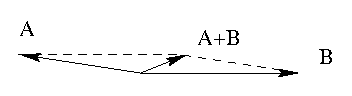
\includegraphics{vectors.eps}
\end{center}

as we can see in this sample (not correlated with the example contained in
the directory) output from troncorb, the orbitals starting from C1C2 are clean
(zero values) in C9 and subsequents. Note also that lines with all zeroes
are removed from the output and there's no order, so it's not impossible to
see all zeroes, then values, then zeroes (take the example of H8):

\begin{verbatim}
 111 C13 2pz    0.0000  0.0000  0.0000  0.0000  0.0000  0.0000  0.0003
-0.0009  0.0013 -0.0029
 112 C13 2pz    0.0000  0.0000  0.0000  0.0000  0.0000  0.0000 -0.0001
-0.0001  0.0005 -0.0004
 113 H8  1s    -0.0006 -0.0862 -0.0512 -0.1060 -0.1601 -0.2420 -0.0422
0.0404 -0.0564 -0.0670
 114 H8  1s    -0.0006 -0.0733 -0.0467 -0.0853 -0.1066 -0.1890  0.0021
-0.0004 -0.0013 -0.0005
 115 H9  1s     0.0000  0.0000  0.0000  0.0000  0.0000  0.0000 -0.0101
0.0507 -0.0374  0.0667
 116 H9  1s     0.0000  0.0000  0.0000  0.0000  0.0000  0.0000  0.0004
-0.0028 -0.0012  0.0005
\end{verbatim}

H8 is not cut out, so is good. This "strangeness" is only for a matter
of numerical ordering.

After the guess production chain ends, we obtain:

from the large calculation

ORTORBG (the orbitals on the large basis)
ORTORBP (the orbitals on the small basis)
MASK (the mask needed to reinsert the ORTORBP inside ORTORBG using expandat)
.Mono -> .Mono.large
.Info -> .Info.large

from the small calculation
.Mono -> .Mono.small
.Info -> .Info.small
.ijcl

Although some stuff is apparently not needed, we need them in order to
obtain correct behaviour of the subsequent optimization procedure.

The optimization procedure is quite tricky and is implemented ad a complex 
bash script. Here i'll report a brief documentation about the routines of
the script.

The available routines are

function checkExists()
  check if a file is available (exists) if does not exists ends the script

function mixInfo()
  accepts 3 parameters: 1) the .Info.large path 2) the .Info.small path 3)
  the resulting output file path.
  This function mix the .Info files from the large calculation and the small
  calculation. For the subsequent optimization procedure we need the .small
  one, but the internal enuc (nuclear energy) must come from the complete
  calculation, since the enuc from the small is corrected with frozen
  orbitals contribution

function mixMono()
  Does the same as above, but on the .Mono.small e .Mono.large. As before
  accepts 3 parameters, and runs the program mixmono with the namelist input
\begin{verbatim}
&MIXMONO
  FILEMONO='$large'
  FILEOVERLAP='$small'
  FILEOUTPUT='$out'
/
\end{verbatim}
  The problem here is that we need to take the mono integrals from the large
  calculation (which cames out from the troncat of the correct size for
  dealing with the small system) but we need the overlap matrix from the
  small calculation. So we need to mix the files since the overlap and the
  monoelectronic integrals are on the same .mono file. A proposal was made
  about splitting these two concepts in two different files (a .Overlap?)
  If the latter is made, mixmono is no longer required and is replaced by a
  simple copy.

function improveOrbitals()
  The main function that does the improvement of the orbitals. Does various
  sanity checks, mix the info and the mono, runs casdet+casdi+locnats and
  produces LOCORB2 as a product (improved orbitals on the small system). Is
  similar to noscf but it works with the new approach

function recreateBi()
  This function recreates the bielectronic MO integrals given the AO
  integrals and the new (hopely improved) orbitals

function recreateMono()
  The same as above, but recreates the monoelectronic MO integrals.

function reinsertOrbitals()
  this function exploit the functionality of expandat to reinsert the
  improved orbitals inside the shell of frozen orbitals. We need this
  reinsertion because we need to recreate the integrals in the MO basis.

function copySewardLarge()
function copySewardSmall()
function copyStartFiles()
function collectOutputFiles()
  utility functions to copy files here and there in the scratch
  to subdivide each iteration, start files and final files in a
  specific directory. 

function extractEnergy()
  grep the energy from the file

function iteration()
  The cyclic function that triggers each iteration workpath

function postProcess()
  A custom function where the post-optimization work is done.
  At the moment we do an cas+sd calculation. This function is triggered
  at convergence (ie. when the energy during the optimization procedure
  produces the same energy with two subsequent evaluations)

due to a software problem, you must also provide a file named SCH\_FERMI
\begin{verbatim}
&ferm fermi= 9, /
\end{verbatim}


\end{document}
